\chapter{Computer Vision}
Computer Vision as a part of machine learning and artificial intelligence, as the name suggests, involves utilizing computation automatization algorithms to analyse and process visual data, like images (2D and 3D) and videos \cite{Szeliski2022, Atallah2020}.

Machine learning is a subset of artificial intelligence, which includes both statistical learning and deep learning algorithms in order to make intelligent decisions about certain data. The modern computer vision belongs to the deep learning part as can be seen in figure \ref{fig:ai-ml}. In classical programming, we are designing a program that produces a desired input for specified types of input. In machine learning however, we let the machine design appropriate program, given the specified set of inputs and outputs (labels) by analysing the features of the input with relation to the output \cite{Alam2021}.

\begin{figure}[H]
\begin{centering}
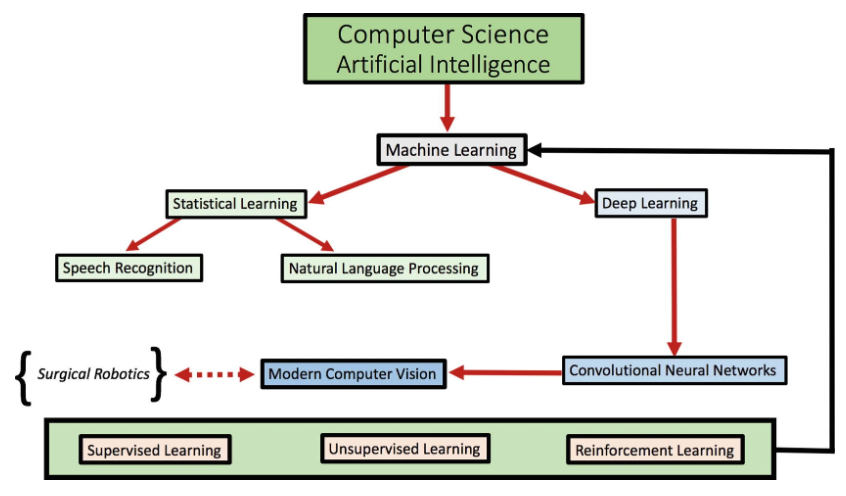
\includegraphics[width=12cm]{assets/images/aiml.png}
\par\end{centering}
\caption{Division of AI/ML \cite{Atallah2020}}
\label{fig:ai-ml}
\end{figure}

With the advent of deep learning \cite{LeCun2015} and especially convolutional neural networks \cite{Ronneberger2015}, the computer vision is now a field of huge interest.

\section{Preprocessing}
Since the machine learning algorithms try to examine the relationship between input and output, we need to ensure an appropriate quality of the input data. Especially in medical imaging and digital histopathology, where the different staining techniques, scanning tools, or position of the tissue can vary widely and this can have affect on the further analysis \cite{Hoque2024}.

In the domain of digital histopathology, a common issue is the varying intensities of purple, red, and pink tones of H\&E stained slides \cite{Hoque2024}. For this purpose different stain normalization techniques were created. Among the examples we can list the Macenko, Reinhart or Zheng normalization techniques, which try to normalize the dataset of input images \cite{Hoque2024}. Among some other techniques we can list the histogram equalization, Contract-Limited Adaptive Histogram Equalization (CLAHE), and the power law (gamma) transformation \cite{Dabass2020}.

\section{Core Computer Vision Tasks}
When analysing an image, we can come across of four main tasks \cite{Alam2021}.

\paragraph{Image Classification}
Image classification is used when we have a label categorizing the image into one of the class (or multiple classes) in the set of classes \cite{Alam2021}. For example in medical imaging domain we could label an image with the "disease" or "non-disease" class .

\paragraph{Object Localization and Object Detection}
Object localization and object detection are very similar tasks. While the former is a task of localizing a single object instance in the image, the later is a task where possible multiple instances of one or many objects should be detected and bounded \cite{Alam2021}.

\paragraph{Segmentation} Sometimes we want to get more detailed label that just an approximate object location (bounding rectangle). Segmentation utilizes pixel-level classification, where pixels can be labelled based on their relationship to various classes. According to \cite{Alam2021} we know two main types of segmentation:

\begin{itemize}
    \item Semantic segmentation, where each pixel of a certain class gets the same label, no matter the number of instances, and
\end{itemize} Instance segmentation, where the pixels of different instances of the same class are distinguished as well.

Example of each of these tasks can be seen in figure \ref{fig:aiml-tasks}.

\begin{figure}[H]
\begin{centering}
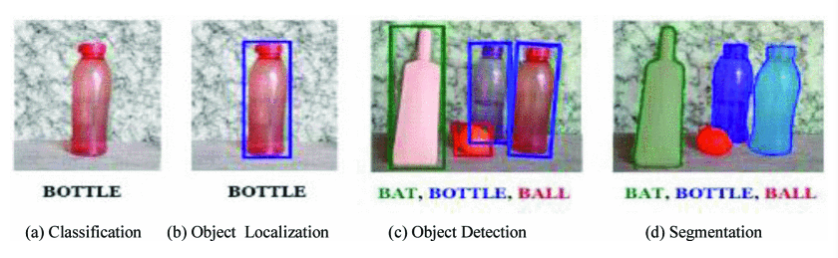
\includegraphics[width=12cm]{assets/images/aiml-tasks.png}
\par\end{centering}
\caption{Different Computer Vision tasks \cite{Alam2021}}
\label{fig:aiml-tasks}
\end{figure}


\section{Learning Paradigms}
Computer vision algorithms can be further divided by how they can learn from the data \cite{Alam2021}.

\paragraph{Supervised Learning} In the supervised learning tasks, both the data and their respective labels are known and are available to the model during the training. Typical supervised learning tasks include classification, detection, and segmentation. By the quality and precision of the labels and the task goal, we can split supervised learning into three categories:

\begin{itemize}
    \item Standard supervised learning, when available labels are of the same quality as the labels we want to predict, e.g. bounding box to bounding box.
    \item Strong supervised learning, when the training labels contain richer information that the labels we want to predict, e.g. bounding box from pixel-level annotations.
    \item Weak supervised learning, when the training labels contain less precise information that the labels we want to predict, e.g. bounding box from image level annotation.
\end{itemize}

\paragraph{Unsupervised Learning} In the unsupervised learning on the other hand, the data labels are not available to the model during the training.
